% Theme-independent poster content. Select a visual theme in
% poster-config.tex or with `make THEME=<theme-name>`.
% Global poster settings. Command-line definitions take precedence, so the
% Makefile can select another theme without editing this file.
\providecommand{\PosterTheme}{lamarr-classic}
\providecommand{\PosterWidth}{61}
\providecommand{\PosterHeight}{85}
\providecommand{\PosterScale}{0.83}


\documentclass[final]{beamer}
\usepackage{posterframework}
\PosterLoadTheme{\PosterTheme}

% ====================
% Title
% ====================

\title{Towards Foundation Models for\PosterTitleBreakA Quantum Unitary Synthesis\PosterTitleBreakB via Zero-Shot MDL}

\author{Lukas Theißinger \inst{1,3} \and Thore Gerlach \inst{2} \and David Berghaus \inst{1,4} \and Christian Bauckhage \inst{1,3,4}}

\institute[shortinst]{\inst{1} Lamarr Institute \samelineand \inst{2} European Space Agency \samelineand \inst{3} University of Bonn \samelineand \inst{4} Fraunhofer IAIS}

% ====================
% Body
% ====================

\begin{document}



\begin{frame}[t]
\begin{columns}[t]
\separatorcolumn

\begin{column}{\colwidth}

	  \begin{block}{Problem setting}
			\begin{itemize}
				\item Given: Target unitary $\mathbf{U}$
				\item Goal: Recover an exact circuit over the Clifford+T gate set
				\item Search: Append one gate at a time until the residual unitary is solved
			\end{itemize}
		
		\begin{figure}
		\begin{tikzpicture}[
			>={Latex[length=7pt,width=9pt]},
			stepbox/.style={rounded corners=3pt,draw=SoftGray,fill=CrispWhite,
				minimum width=5cm,minimum height=3.8cm,inner sep=2pt},
				steplabel/.style={font=\normalsize,text=Aqua},
				gatelabel/.style={font=\normalsize,align=center,fill=CrispWhite,inner xsep=4pt,inner ysep=1pt}
				]
			\node[stepbox] (c0) {};
			\node[stepbox,right=1.43cm of c0] (c1) {};
			\node[stepbox,right=1.43cm of c1] (c2) {};
			\node[stepbox,right=1.43cm of c2] (c3) {};

			% Draw the circuit states directly so the poster has no generated-file
			% dependency for this small schematic.
			\foreach \c in {c0,c1,c2,c3} {
				\node[font=\small,anchor=west] at ($(\c.west)+(0.12cm,0.55cm)$) {$q_0$};
				\node[font=\small,anchor=west] at ($(\c.west)+(0.12cm,-0.55cm)$) {$q_1$};
				\draw[SoftGray,line width=1.1pt] ($(\c.west)+(1.05cm,0.55cm)$) -- ($(\c.east)+(-0.25cm,0.55cm)$);
				\draw[SoftGray,line width=1.1pt] ($(\c.west)+(1.05cm,-0.55cm)$) -- ($(\c.east)+(-0.25cm,-0.55cm)$);
			}
			\foreach \c/\x in {c1/0.45,c2/-0.10,c3/-0.70} {
				\fill[Aqua] ($(\c.center)+(\x cm,0.55cm)$) circle (2.3pt);
				\draw[Aqua,line width=1.2pt] ($(\c.center)+(\x cm,0.55cm)$) -- ($(\c.center)+(\x cm,-0.55cm)$);
				\draw[Aqua,line width=1.2pt] ($(\c.center)+(\x cm,-0.55cm)$) circle (0.22cm);
				\draw[Aqua,line width=1pt] ($(\c.center)+(\x cm,-0.77cm)$) -- ($(\c.center)+(\x cm,-0.33cm)$);
				\draw[Aqua,line width=1pt] ($(\c.center)+(\x cm-0.22cm,-0.55cm)$) -- ($(\c.center)+(\x cm+0.22cm,-0.55cm)$);
			}
			\node[draw=Aqua,line width=1.1pt,fill=CrispWhite,minimum size=0.6cm]
				at ($(c2.center)+(0.85cm,-0.55cm)$) {$T$};
			\node[draw=Aqua,line width=1.1pt,fill=CrispWhite,minimum size=0.6cm]
				at ($(c3.center)+(0.15cm,-0.55cm)$) {$T$};
			\fill[Aqua] ($(c3.center)+(1.00cm,0.55cm)$) circle (2.3pt);
			\draw[Aqua,line width=1.2pt] ($(c3.center)+(1.00cm,0.55cm)$) -- ($(c3.center)+(1.00cm,-0.55cm)$);
			\draw[Aqua,line width=1.2pt] ($(c3.center)+(1.00cm,-0.55cm)$) circle (0.22cm);
			\draw[Aqua,line width=1pt] ($(c3.center)+(1.00cm,-0.77cm)$) -- ($(c3.center)+(1.00cm,-0.33cm)$);
			\draw[Aqua,line width=1pt] ($(c3.center)+(0.78cm,-0.55cm)$) -- ($(c3.center)+(1.22cm,-0.55cm)$);
			
			\node[steplabel,below=2pt of c0] {start};
			\node[steplabel,below=2pt of c1] {1 gate};
			\node[steplabel,below=2pt of c2] {2 gates};
			\node[steplabel,below=2pt of c3] {3 gates};
			
			\draw[-Latex,line width=1.6pt,Aqua] (c0.east) -- (c1.west);
			\draw[-Latex,line width=1.6pt,Aqua] (c1.east) -- (c2.west);
			\draw[-Latex,line width=1.6pt,Aqua] (c2.east) -- (c3.west);
				
			\node[gatelabel] at ($(c0.east)!0.5!(c1.west)+(0,2.45cm)$) {\shortstack{\textcolor{SoftGray}{I}\\\textcolor{SoftGray}{S}\\\textcolor{SoftGray}{H}\\\textcolor{SoftGray}{T}\\{\color{Aqua}\bfseries CX}}};
			\node[gatelabel] at ($(c1.east)!0.5!(c2.west)+(0,2.45cm)$) {\shortstack{\textcolor{SoftGray}{I}\\\textcolor{SoftGray}{S}\\\textcolor{SoftGray}{H}\\{\color{Aqua}\bfseries T}\\\textcolor{SoftGray}{CX}}};
			\node[gatelabel] at ($(c2.east)!0.5!(c3.west)+(0,2.45cm)$) {\shortstack{\textcolor{SoftGray}{I}\\\textcolor{SoftGray}{S}\\\textcolor{SoftGray}{H}\\\textcolor{SoftGray}{T}\\{\color{Aqua}\bfseries CX}}};
		\end{tikzpicture}
		\caption{Example synthesis task for $\mathbf{U} = \operatorname{diag}(1,e^{i\pi/4},e^{i\pi/4},1)$: recover the exact 3-gate circuit $\mathrm{CX}_{01} T_1 \mathrm{CX}_{01}$. Blue labels show the selected gate at each step}
		\end{figure}
    
  \end{block}

  \begin{block}{Challenges}
	    \begin{itemize}
	      \item The problem is NP-hard in general
	      \item Search space grows exponentially with the length of the circuits
	      \item Standard unitary distances do not provide reliable search guidance
	    \end{itemize}

		\begin{figure}
			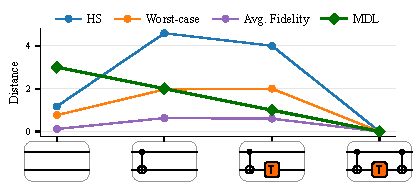
\includegraphics[width=0.95\textwidth,height=0.589\textheight,keepaspectratio]{gfx/teaser_figure.pdf}
					\caption{Along the correct path, Hilbert-Schmidt, worst-case and average-fidelity error are non-monotone, while MDL drops cleanly from 3 to 0.}
		\end{figure}

  \end{block}

  \begin{posterfeatureblock}{Minimum description length (MDL)}
	  	\begin{itemize}
	  		\item \textbf{MDL principle:} Prefer the shortest exact explanation
			\item \textbf{For synthesis:} MDL is the remaining gate count of the shortest exact circuit
			\item \textbf{Search view:} Along a correct path, MDL decreases by one per step
			\item \textbf{Challenge:} Exact MDL is NP-hard, so we learn a predictor instead
	  	\end{itemize}
	   
  \end{posterfeatureblock}
  
  \begin{block}{Training MDL Predictor}
	  	\begin{itemize}
	  		\item \textbf{Generate circuits} Sample Clifford+T circuits on the fly and rebalance the dataset across $T$-counts
	  		\item \textbf{Build labels} Run a fast optimizer; the optimized suffix length becomes the approximate MDL target. For harder targets, also include easier partial circuits
	  		\item \textbf{Train predictors} Phase-normalize the unitary and train either an MLP on matrix entries or a Transformer on tokenized inputs
	  		\item \textbf{Loss} Regress the scalar MDL target with MSE
	  	\end{itemize}
  \end{block}
  
  \begin{block}{Inference: Stochastic Beam Search}
  	\begin{itemize}
  		\item Couple MDL Predictor with Beam search
  		\item Rank partial circuits by predicted remaining MDL
  		\item Beam search is fast and highly parallelizable
  		\item Add stochasticity and equivalent root states to improve exploration
  	\end{itemize}
 \end{block}	
  
  %\begin{block}{References}
  %	\scriptsize
 % 	\setlength{\parskip}{0.15em}
 % 	\begin{minipage}[t]{0.48\linewidth}
 % 		\raggedright
 % 		[1] B.~Giles and P.~Selinger. \emph{Exact synthesis of multiqubit Clifford+T circuits}. Phys. Rev. A, 2013.\par
 % 		[2] V.~Kliuchnikov, D.~Maslov, and M.~Mosca. \emph{Fast and efficient exact synthesis of single-qubit unitaries generated by Clifford and T gates}. QIC, 2013.\par
 % 		[3] M.~Amy et al. \emph{A meet-in-the-middle algorithm for fast synthesis of depth-optimal quantum circuits}. IEEE TCAD, 2013.\par
 % 		[4] J.~van de Wetering and M.~Amy. \emph{Optimising quantum circuits is generally hard}. arXiv, 2023.
 % 	\end{minipage}\hfill
 % 	\begin{minipage}[t]{0.48\linewidth}
 % 		\raggedright
 % 		[5] S.-X.~Zhang et al. \emph{Differentiable quantum architecture search}. Quantum Sci. Technol., 2022.\par
 % 		[6] X.~Lu et al. \emph{QAS-Bench: Rethinking quantum architecture search and a benchmark}. ICML, 2023.\par
 % 		[7] A.~Paradis et al. \emph{Synthetiq: Fast and versatile quantum circuit synthesis}. Proc. ACM Program. Lang., 2024.\par
 % 		[8] S.~Rietsch et al. \emph{Unitary synthesis of Clifford+T circuits with reinforcement learning}. QCE, 2024.
 % 	\end{minipage}
 % \end{block}

\end{column}

\separatorcolumn

\begin{column}{\colwidth}
		\begin{posterfigureblock}{Beam search view}
		\begin{figure}
			\centering
			\includegraphics[width=0.67\textwidth]{\PosterInferenceTree}
			\caption{Beam-search view: candidate partial circuits are expanded, ranked by predicted remaining MDL, and pruned back to the beam}
		\end{figure}
		\end{posterfigureblock}
		
	
		\begin{postertakeaways}{Takeaways}
			\normalsize
			\textbf{A simple and reusable, {\color{TakeawayAccent}zero-shot} MDL-guided search heuristic for quantum unitary synthesis that is cheap to train and fast at inference}
			\vspace{0.5em}
			
			\centering
			\statcallout{6 h vs.\ 7 d}{MLP training cost versus the reported RL baseline}
			\hfill
			\statcallout{22 s}{average runtime per 5-qubit instance at test time}
			\hfill
			\statcallout{15/15}{successes in almost every QAS-Bench bucket}
			\end{postertakeaways}

				\begin{block}{Results}
					{\normalsize \textbf{QAS-Bench} standardized Benchmark. Testing on 2--5 qubits, difficulty levels 1--6 with 15 targets per bucket.
						We solve nearly every bucket 15/15 and beat \texttt{Synthetiq} on the hard multi-qubit cases.\par}
						\vspace{0.8em}
						\noindent\makebox[\linewidth][c]{%
							\comparepanel{gfx/QASHeatmaps/qas_success_heatmap_synthetiq.png}{Synthetiq}%
						\hfill
						\comparepanel{gfx/QASHeatmaps/qas_success_heatmap_beam_099.png}{Ours}%
					}\par
						\vspace{0.4em}
						
						{\normalsize \textbf{Random targets} Success degrades more slowly as the $\mathbf{T}$-count increases in comparison to RL.\par}
					
					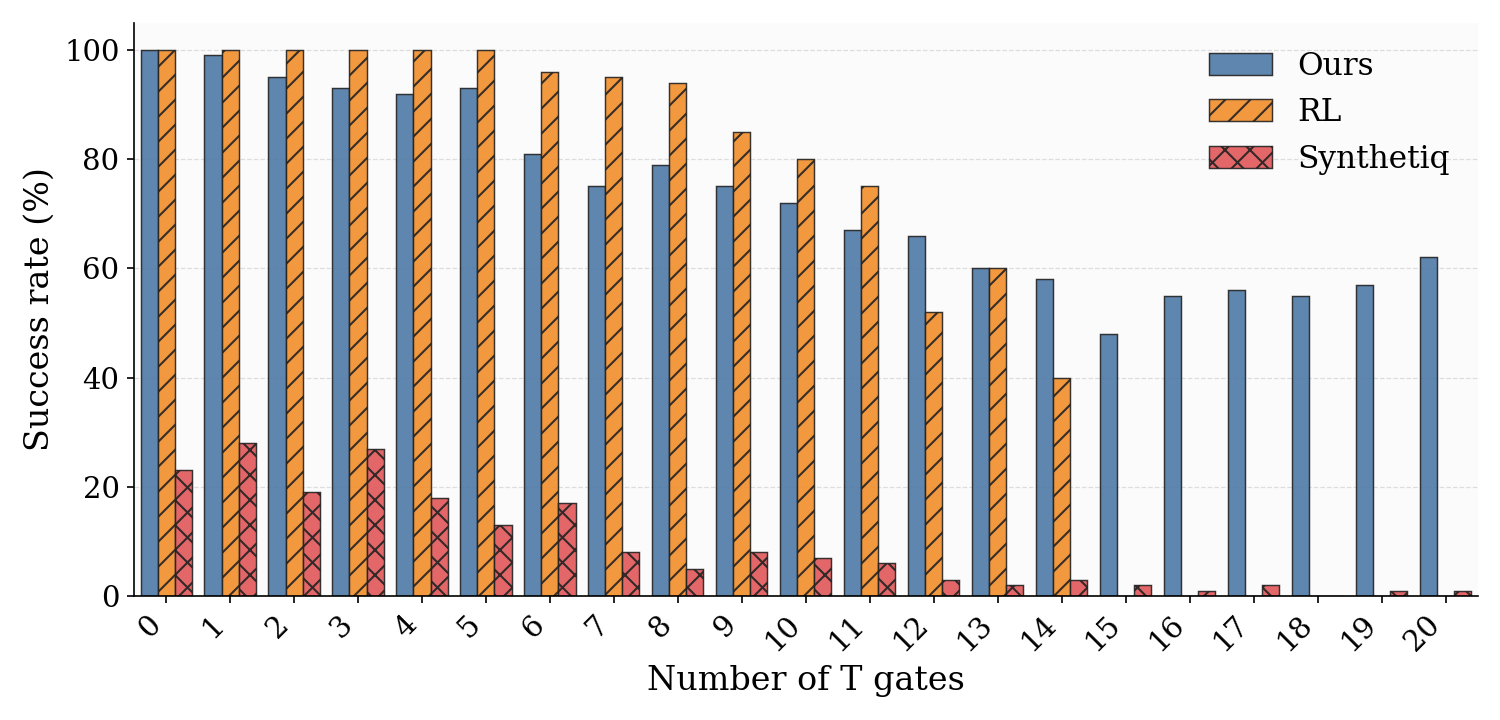
\includegraphics[width=0.86\linewidth]{gfx/results/histogram_comparison_5.png}
					
					{\scriptsize RL bars are only approximate. Additional comparisons can be found in the paper}
				\end{block}

		\begin{block}{Limitations}
			\begin{itemize}
				\item Search states are dense $2^n \times 2^n$ matrices, so memory still scales as $\Theta(4^n)$
				\item Performance depends on the training distribution
				\item Beam search trades compute for quality and has no worst-case guarantee
				\item Cannot be used directly with parametric gate sets
			\end{itemize}
	\end{block}
  
\end{column}

\separatorcolumn
\end{columns}
\end{frame}

\end{document}
